\section{Time evolution operator of the system}

We start from the simplest situation; a time independent Schr$\ddot{\mbox{o}}$dinger equation,

\begin{equation*}
    i \hbar \frac{\partial }{\partial t} | \psi \rangle = H | \psi \rangle
\end{equation*}

In Schr$\ddot{\mbox{o}}$dinger picture, where the operators are time dependent,
We can express a solution of $|\psi(t) \rangle$ with unitary operator, $U$,
\begin{equation}
    \label{eq:time_inde_sol}
    |\psi(t)\rangle = U(t) | \psi(0)\rangle 
\end{equation}

What we have at the initial stage were an initial state and the given Hamiltonain.
From the information, we have to get a $U(t)$ operator for simulate
the dynamics of the given system.
The solution of Eq (\ref{eq:time_inde_sol}) is achieved easily 
if the $H$ has no time dependency\footnote{
    In general, the solution is never gone like the Eq (\ref{eq:time_inde_sol}). 
    We will see it in a further section.}.

\begin{equation}
    U(t) = \exp( -i \frac{1}{\hbar} (H) t)
\end{equation}

A more precise notation is $U(t_i, t_f)$ which indicates the initial time and final time.
With the notation, the $U(t)$ is $U(0, t)$.
We call it as a time-propagator\footnote{
    In mathematics, such propagator is a green function of solution of differential or integral equations.
    $G(s_n, t_n | s_0, t_0) = U(t_n, t_0)$
}
Here is why the gate model is called a discrete computation model.
It is because we cannot directly implement the such general time-propagator 
per each system. Only thing we can manipulate is just an approximation 
of the propagator with basic block gates. 
Fortunately, the universal gate set to represent approximate all unitary operator
is well investigated. See \textit{Solovay-Kitaev theorem}.
\index{Solovay!Solovay-Kitaev theorem}
\index{Kitaev!Solovay-Kitaev theorem}


\begin{definition}\textbf{Unitary approximation}
    For a given unitary gate, $U(t)$, 
    approximation of $U(t)$ is a constructing an $U'(t)$ gate 
    which consist of the universal gate set of the quantum machine,
    such that minimize the next,

    \begin{equation}
        \max\left(|U(t) - U'(t)|\right)
    \end{equation}
\end{definition}

%---------------------------------

\begin{marginfigure}
    \centering
    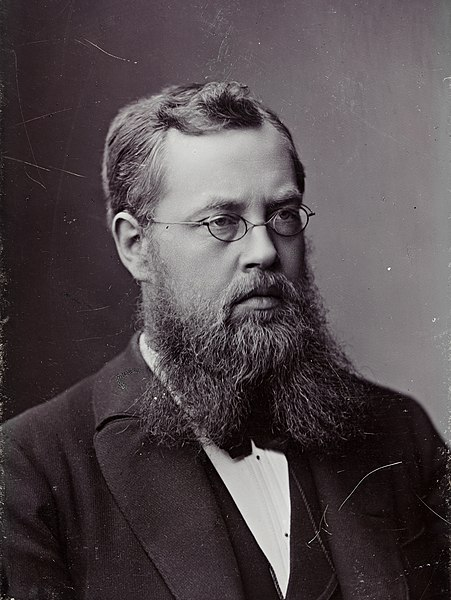
\includegraphics[width=0.6\textwidth]{media/picture_Sophus_Lie.jpg}
    \caption{Sophus Lie}
    \label{fig:sopus_lie_picture}
\end{marginfigure}
\index{Lie}
\index{Sophus Lie}

Then, what we need? What does the operator mean inside of exponential?
It is called exponential mapping of operator, and 
it plays a key concept of time-evolution in quantum mechanics.
The major properties and definiton were first investigated by \textit{Sophus Lie} with his research on continuous group and 
differential geometry.
It has tremendous interesting properties and applications in both physics and mathematics.
However, in here, we only look up 
the operator map for evolution implementation in finite matrix group.

\subsection{Exponential Map}

\begin{definition}{\textbf{Operator exponential}}
    \index{Operator Exponential}
    \begin{equation}
        \exp(\hat{X}) = \sum_{k=0} \frac{1}{k !} \hat{X}^k
    \end{equation}
\end{definition}

The map is converges $\forall X \in \mathbf{M}_{n}(\mathbb{C})$.

\begin{theorem} \textbf{Properties of Exponential Map}
    \begin{itemize}
        \item $e^X$ is a continuous function.
        \item $e^0 = I$
        \item $(e^X)^\ast = e^{X^\ast}$
        \item $e^X$ is always invertible, and $(e^X)^{-1} = e^{-X}$.
        \item $e^{(a+b)X} = e^{aX} e^{bX}$.
        \item If $[X, Y] = 0$, $e^{X+Y} = e^{X}e^{Y} = e^{Y}e^{X}$.
        \item $\forall M \in \text{GL}(n; \mathbb{C}), e^{M X M^{-1}} = M e^{X} M^{-1}$. 
    \end{itemize}
\end{theorem}

If $\hat{A}$ was a digonal matrix, then the next relationship hold.

\begin{equation*}
    A = \begin{bmatrix}
        \lambda_1 & 0 & \dots & 0 \\
        0 & \lambda_2 & \dots & 0 \\
        \vdots & 0 & \ddots & \vdots\\
        0 & 0 & \cdots & \lambda_n
    \end{bmatrix},
    e^A = \begin{bmatrix}
        e^{\lambda_1} & 0 & \dots & 0 \\
        0 & e^{\lambda_2} & \dots & 0 \\
        \vdots & 0 & \ddots & \vdots\\
        0 & 0 & \cdots & e^{\lambda_n}
    \end{bmatrix}
\end{equation*}

In general not only for the digonal matrix, 
the exponential map preserves the eigenvectors of the original matrix.

\begin{exercise}
    For an eigen vector, $\mathbf{v}$, of the given matrix, $X$, with eigenvalue, $\lambda$,

    \begin{equation}
        X \mathbf{v} = \lambda \mathbf{v}
    \end{equation}

    Show that 

    \begin{equation*}
        e^X \mathbf{v} = e^\lambda \mathbf{v}
    \end{equation*}
\end{exercise}

In general case, we decompose the Hamiltonian as sum of local terms,
and the time as sum of many intermediate steps.
These slicing allow us to analysis the dynamics of the system evolution
in specific local region or local time. 
First, the time slicing is not different with usual exponential function.
The time-propagator from time $t_0$ to $t_n$ can be decomposed to 
$n$ intermediate step propagators,

\begin{eqnarray*}
    U(t_n, t_0) &= U(t_0 + \Delta t, t_0) U(t_0 + 2\Delta t, t_0 + \Delta t) \cdots U(t_n, t_n - \Delta t) \\
                &= \Pi_{i=0}^{n-1} U(t_{i+1}, t_i)\\
                &= \Pi_{i=0}^{n-1} \exp \left( - i \Delta t H\right)\\
                &= \exp \left( - i (t_n - t_0) H\right)\
\end{eqnarray*}

However, decomposition with local Hamiltonian, $H = \sum_k H_k$ yields 
a problem. The non-commuting terms in $\sum_k H_k$ makes an error in the expotential map.

\begin{align*}
    [H_i, H_k] \neq 0\\
    e^{H_i + H_k} \neq e^{H_i} e^{H_k} \, \text{ or } \, e^{H_k} e^{H_i}
\end{align*}

Major problem arises in here. 
Since, we cannot directly implement the given evolution gate, 
but just applying sequential local term does not yield
the correct gate. The problem would be investigated in the following 
subsection. 

\subsubsection{Pauli matrix and exponential}

Before, we move to the non-commuting problem. 
Let us see basic properties of Pauli matrices as a basis set of matrix space.
In the above paragraph, we read the Hamiltonian could be decomposed 
into several local Hamiltonians. 
Mostly, we decompose them with Pauli matrices.
Since, Pauli matrices have good properties to decompose 
the general Hamiltonian. 

\begin{definition}\textbf{Pauli matrices}
    \index{Pauli matrices}
    \begin{equation}
        \sigma_0 = \begin{bmatrix}
            1 & 0 \\
            0 & 1
        \end{bmatrix},
        \sigma_1 = \begin{bmatrix}
            0 & 1 \\
            1 & 0
        \end{bmatrix},
        \sigma_2 = \begin{bmatrix}
            0 & -i \\
            i & 0
        \end{bmatrix},
        \sigma_3 = \begin{bmatrix}
            1 & 0 \\
            0 & -1
        \end{bmatrix}
    \end{equation}
\end{definition}

Usually, $\sigma_X = \sigma_1, \sigma_Y = \sigma_2, \sigma_Z = \sigma_3$.
By the context, the notation could be different. Sometime just only use $X, Y, Z$.

\begin{exercise}
    Show that, 
    \begin{equation*}
        [\sigma_j, \sigma_k] = 2 i \epsilon_{jkl} \sigma_l
    \end{equation*}
    and
    \begin{equation*}
        \sigma_j \cdot \sigma_k = \delta_{jk} I + i  \epsilon_{jkl} \sigma_l
    \end{equation*}
\end{exercise}

First, it forms a complete orthonormal basis in matrix space,
with Hilbert-Schmidt inner product.

\begin{definition}\textbf{Hilbert-Schmidt inner product}\index{Hilbert-Schmidt inner product}
    For two given matrices, $A, B \in \mathbf{M}(\mathcal{C})$,
    Hilbert-Schmidt inner product of two matrices is,

    \begin{equation}
        \langle A | B \rangle_{HS} := \frac{1}{N}\text{Tr}(A^\dagger B)
    \end{equation}
\end{definition}

The $1/N$ is a normalization factor. 

\begin{exercise}
    Prove that the Hilbert-Schmidt inner product satisifes inner product axiom.

    \begin{itemize}
        \item Positive definiteness: $\langle X | X \rangle \geq 0$.
        \item Linearity: $\langle a X+ bY | Z \rangle = a \langle X | Z \rangle + b \langle Y | Z \rangle$.
        \item Conjugate symmetry: $\langle X | Y \rangle = \overline{\langle Y | X \rangle}$
    \end{itemize}
\end{exercise}

\begin{exercise}
    Show that any 2-by-2 square matrix can be decomposed into sum of Pauli matrices 
    and it forms an orthonormal basis set of 2-by-2 matrices vector space.
\end{exercise}

Second, usual quantum computing systems are based on spin system.
Therefore, Pauli and their generalized gates are universal for most quantum computing frameworks
\footnote{There are some exceptions, but in those systems, we can still use Pauli gates.}.
Third, the algebra of Pauli matrices is well studied so that the manipulation framework has been well established.
Pauli decomposition allow us to deal the given Hamiltonian as an algebraic object.

The best operators to represent the Hamiltonian are unitary \textbf{and} simultaneously Hermit operators. 
If the given operator, $\hat{A}$ is unitary and hermit then, the next relationship is hold,
\begin{equation}
    \hat{A} = \exp(i \frac{\pi}{2}\hat{A}).
\end{equation}

Pauli-matrices, $\sigma_{X}, \sigma_{Y}, \sigma_{Z}$, are typical example of the such matrix.
It is unitary, Hermit, and complete orthonormal basis set. 
In $2^n>2$, Hilbert space, their tensor product also hold the properties.
Therefore, any given Hamiltonian of $2^n \times 2^n$ dimension matrix can be expressed with $n$-length Pauli-string, 
$P^n$

\begin{equation}
    \label{eq:Pauli-decompositon}
    \mathcal{H} = \sum_i^l \mathcal{H}_i = \sum_j^{2^n} \lambda_j P_j^n
\end{equation}
where, $P_j^n$ is a representing an element of $n$-folded Pauli matrices.
For example, $P_1^3 = XYX$ is a $\sigma_X \otimes \sigma_Y \otimes \sigma_X$. 

Somtimes we denote the Hamiltonian as vector notation whose basis is Pauli group.

\begin{equation}
    \begin{split}
        H = H \cdot \hat{\mathbf{\sigma}} \\
        c_0 \sigma_0 +c_1 \sigma_1+c_2 \sigma_2+c_3 \sigma_3
    \end{split}
\end{equation}

\begin{exercise}
    Suppose that basis of vectros is Pauli group.

    Find a coefficient formula of inner product of two vector
    where the inner product of two vector, $v, w$ 
    is defined as
    
    \begin{equation*}
        \begin{split}
            v = \sum_{i=0}^3 a_i \hat{\sigma}_i \\
            w = \sum_{i=0}^3 b_i \hat{\sigma}_i \\
            v \cdot w = \sum_{j, k} a_j b_k (\hat{\sigma}_j \cdot \hat{\sigma}_k)
        \end{split}
    \end{equation*}

    and so do on outter product.

    \begin{equation*}
        v \times w = \sum_{j, k} a_j b_k (\hat{\sigma}_j \times \hat{\sigma}_k)
    \end{equation*}
\end{exercise}

One thing you have to notice is that the coefficient $\lambda_j$ are all real valued.
It is a spectrum theorem for Hermit matrix. See Theorem \ref{theorem:hermit_spectrum} in Appendix \ref{appendix_chap:hermit_uni}.
It is because the complex valued linear combination does not preserve the hermiticity of the 
summation. You can check yourself with verify the $H_3 = H_1 + i H_2$, whether $H_3$ satisfies hermiticity or does not
when $H_1$ and $H_2$ were Hermit matrices.

\subsection{Problem of commutation}

Now, we have a practical formula for calculating 
the evolution operator of the given Hamiltonain.
Where was a difficulty to implement the evolution operator on the circuit?
The problem arise when the local terms are not commute each other in Eq (\ref{eq:Pauli-decompositon}).
It is common if they are operators, matrices, or more widely general group elements.
We are familiar with commutation group, Abelian group, however, for operators it is not common.
For example, if they are commuting group element, typical example is real or complex number field; $\mathbb{R, C}$. 
About the $x, y \in (+, \times, \mathbb{R} \mbox{ or } \mathbb{C})$, 

\begin{equation}
    \exp(x) \exp(y) = \exp(y) \exp(x) = \exp(x+y)
\end{equation}

holds true. However, such expression does not hold in general case and moreover, 
$\exp(x)\exp(y) = \exp(z)$ solution may not exist.

For example, in matrix group, $\mathbf{M}_2 (\mathbb{C})$,

\begin{eqnarray}
    X = \begin{pmatrix}
        0     & i \pi \\
        i \pi & 0 
    \end{pmatrix}, 
    Y = \begin{pmatrix}
        0     & 1 \\
        0     & 0 
    \end{pmatrix} \\
    \exp(X) \exp(Y) =  
    \begin{pmatrix}
        -1  & 0 \\
        0   & -1 
    \end{pmatrix}
    \begin{pmatrix}
        1 & 1 \\
        0 & 1 
    \end{pmatrix} =
    \begin{pmatrix}
        -1     & -1 \\
        0 & -1 
    \end{pmatrix} = \exp(Z) \label{eq:non-exist-expz}
\end{eqnarray}
$Z$ satisfying $\exp(Z)$ does not exist
\cite{hall2015lie}\footnote[4]{
    \textit{This is a Example 3.41 on page 67}.
}. The exponential map is defined on whole $\text{GL}(n, \mathbb{C})$, however, 
it is not surjective.

However, at least, the $\Pi_k \exp\left(H_k\right)$
seems appropriate for starting point to be closed to
to $\exp\left( \sum_k H_k \right)$.
Then, how much gap between the two operators? and
how can we reduce the gap?
What relationship do they have including non-commutting local terms?
It is represented with \textit{BCH formula}\cite{suzuki_convergence_1977}.
\index{Baker-Campbell-Hausdorff formula}
\index{BCH-formula}

\begin{theorem} \textbf{Baker-Campbell-Hausdorff formula}
    \label{theorem:BCH}
    For the next equation, 
    \begin{equation*}\exp(X) \exp(Y) = \exp(Z)\end{equation*}

    the solution $Z$ is,

    \begin{equation}
        Z = X + Y + \Theta([X, Y]) .
    \end{equation}

    where, $\Theta([X, Y])$ is an error terms as
    
    \begin{eqnarray}
        \Theta([X, Y]) &=& \frac{1}{2}[X, Y] + \frac{1}{12} [[X, Y], Y-X] + \dots \\
        &=& \sum_n^\infty \frac{1}{n!} \left[\frac{\partial^n}{\partial \lambda^n} \ln \sum_{k=0}^\infty \sum_{j=0}^\infty  \frac{\lambda^{k+j}}{k! j!} X^k Y^j \right]_{\lambda = 0} .
    \end{eqnarray}
\end{theorem}

The BCH theorem provides us a reason why there is no solution $Z$ in Eq(\ref{eq:non-exist-expz}).
It hardly depends on the properties of $X, Y$ operators.
The direction is clear now. 
The $\exp(X)\exp(Y)$ does not exactly same with $\exp(X+Y)$ but, if $O(X, Y)$ term converges to finite value,
It would be a good approximation of the original evolution.
Suzuki analyzed convergence conditions of the BCH formula\cite{suzuki_convergence_1977}.

\begin{theorem} \textbf{Convergence of BCH formula 1}

    The BCH formula converges for $(||A|| + ||B||) < \ln2$    
\end{theorem}
where, $||\cdot||$ is Hilbert-Schmidt norm.

\begin{definition} \textbf{Hilbert-Schmidt norm} % Encyclopedia of mathematics, cite

    About the matrix, $A$ over field $\mathbb{F}$, Hilbert-Schmidt norm is 
    \begin{equation*}
        ||A|| := \sqrt{\sum_{i \in I} ||Ae_i||^2}
    \end{equation*} 
    where, $\{e_i\}_{i \in I}$ is an orthnormal basis.
\end{definition}

Simply, we can rewrite the above norm as

\begin{equation}
    ||A|| = \sqrt{\sum_{i j} ||a_{ij}||^2} = \sqrt{\text{Tr} (A^\ast A)}
\end{equation}

\begin{theorem} \textbf{Convergence of BCH formula 2}
    \label{theorem:converges_BCH_2}
    
    For any set of operators $A$ and $B$ in a Banach algebra, the expansion $W$ in
    \begin{eqnarray}
        \exp(A + B) = \exp(A) \exp(B) \exp(W) \\
        W = \sum_{n=2}^\infty W_n
    \end{eqnarray}

    converges, at least, for
    \begin{equation}
        (||A|| + ||B||) < \frac{1}{2} \ln 2
    \end{equation}
\end{theorem}


\begin{exercise}
    The definition of Banach algebra is 
    \begin{definition}\textbf{Banach Algebra}
        For the complete normed space $(X, ||\dot||)$ and $x, y \in X$, the 
        \begin{equation*}
            ||xy || \leq ||x|| ||y||
        \end{equation*}
    \end{definition}

    Show that with Hilbert-Schmidt norm, the matrix space over field $\mathbb{C}$ 
    satisfies Banach Algebra.
\end{exercise}
Since, \textbf{separable} Hilbert space satisfies the Banach Algebra axioms and every finite Hilbert space are separable.
Therefore, we can freely use the above convergence formula for finite qubit-system.

This property generate errors, $\Theta(X, Y)$, between the true evolution operator 
and the product of exponentials of each Pauli-string component. 

\begin{equation}
    U = \exp(\mathcal{H}_i \Delta t) \neq \Pi \exp(\lambda_i P_i^n \Delta t)
\end{equation}

It is not exactly same with the correct unitary operator, 
however, we can approximate it to the operator by slicing of time unit.
It is a \textit{Product Formula}.

\begin{theorem} \textbf{Product Formula}
    
    \begin{equation*}
        \label{eq:product_formula}
        \exp(X + Y) = \lim_{n \rightarrow \infty} \left(\exp(X/n) \exp(Y/n)\right)^{n} 
    \end{equation*}
\end{theorem} \index{Product Formula}

The error bound is $O(t^2)$ for the evolution time $t$, thus

\begin{equation}
    \exp(tA) \exp(tB) = \exp(t(A+B) + O(t^2))
\end{equation}

It was originally used in Monte-Carlo simulation for quantum system 
and was adopted in QC by Llyod\cite{lloyd_universal_1996}.

%===
\index{Product Formula!Trotter}
\index{Product Formula!Lie-Trotter}
\index{Product Formula!Trotter-Suzuki}
%===
Let us, analysis the above equation, $\exp(X/n) \exp(Y/n)$ guarantees that whatever $||X||+||Y||$ value it is, there exists $N$ such that 
$\forall n >N, \, \frac{1}{n}(||X|| + ||Y||) < \ln(2)$ which satisfies the Theorem \ref{theorem:converges_BCH_2}.
In addition, for $Z$ satisfies $\exp(X/n)\exp(Y/n) = \exp(Z)$, $\Pi_{i=1}^n \exp(Z) = \exp(n Z)$ because every operator commute with itself.

Generally, for $\mathcal{H} = \sum \mathcal{H}_i$,
\begin{equation}
    \exp(- i t \mathcal{H}) = \lim_{n \rightarrow \infty} \left( \Pi_{i=1}^n \exp(-i \frac{t}{n} \mathcal{H}_i) \right)^n
\end{equation}

As an approximation, the time, $T$ evolution of the given Hamiltonian, $\mathcal{H}$ can be modeled as

\begin{equation}
    \exp(-i \mathcal{H} T) \approx [\exp(-i \mathcal{H} \Delta t)]^{T/(\Delta t)}
\end{equation}
where, $n= T/(\Delta t)$ is called Trotter number.
This technique is sometimes noted by \textit{Suzuki-Trotter expansion} of 1st kind, ST1.
There is a better error bound expansion, we call ST2 and further.

\subsection{Suzuki Trotter expansion}

This method is called by \textit{Fractal decomposition}\index{Fractal decomposition}\cite{suzuki_finding_2005}.


\begin{theorem}\textbf{2nd order Suzuki Trotter expansion}
    \begin{equation}
        \label{eq:2nd_suzuki}
        \exp\left(t (F + G)\right) \approx [\exp(F \frac{\Delta t}{2}) \exp(G\Delta t) \exp(F \frac{\Delta t}{2})]
    \end{equation}
\end{theorem}

With second order ST expansion, the error rate is $O(t^3)$.

Generally, the $H = \sum_k H_k$ term Hamiltonian could be expanded with ST2 expansion formula,

\begin{equation}
    e^{-i H t} \approx \left( e^{-i H_1 t/2} e^{-i H_2 t/2} \cdots e^{-i H_n t/2} \right)\left(e^{-i H_n t/2} \cdots e^{-i H_2 t/2} e^{-i H_1 t/2} \right)
\end{equation}

Be aware the oreder of the local Hamiltonians, in the 1st term, the order is ascending but, in the 2nd term
it is descending order. It is a recursive formula of Eq (\ref{eq:2nd_suzuki}).

For the higher expansion, it is defined with recursively

\begin{theorem} \textbf{n-th order ST expansion}
    \label{theorem:n_ST}
    \begin{equation}
        S_{2n+2}(t; A, B) = S_{2n}(s_{2n} t; A, B)^2 S_{2n}((1-4s_{2n}) t; A, B) S_{2n}(s_{2n} t; A, B)^2 
    \end{equation}

    where, $S_2(t; A, B)$ is 

    \begin{equation}
        S_2(t; A, B) = e^{t A/2} e^{t B} e^{t A/2}
    \end{equation}

    and the error is $O(t^{2n+3})$ when 

    \begin{equation}
        s_{2n} = \frac{1}{4 - {}^{2n+1}\sqrt{4}}
    \end{equation}
\end{theorem}

However, mostly we only use ST1, Eq (\ref{eq:product_formula}), or ST2 method.
We can make a precise approximation quantum gate following Theorem \ref{theorem:n_ST},
but the total number of terms are too long considering the computational resource, 
even in the quantum computer.

The BCH formula could be used for proving \textbf{Stone-von Neumann Theorem},
it is a different notation of Canonical Conjugation Relationship(CCR) of two observables.
Since, the some modeling Hamiltonians are based on CCR observables,
the theorem is worth to note here.

\subsubsection{Stone-von Neumann Theorem}

\begin{theorem}  % See Quantum Theory for Mathematicians
    For two Hermit operators satisfying canonical commutation relation, 
    $[X, P] = i I$,
    and $a, b \in \mathbb{R}$
    
    \begin{equation}
        e^{i a X} e^{i b P} = e^{- i ab} e^{i bP} e^{iaX}
    \end{equation}
\end{theorem}

This is a Weyl's version of CCR, where the original form in QM was,

\begin{equation}
    [x, p] = i \hbar
\end{equation}

The proof could be started from BCH formula, applying $[X, Y] = i \hbar I$.
The error term $O(X, Y)$, in fact, depends on their commutator, $[X, Y]$, 
so that $O(X, Y) = O([X, Y])$\cite{PhysRevX.11.011020}. 
With ST2, the next relationship hold for $[X, P] = i\hbar I$.

\begin{equation}
    \exp(i (a X + b P)) = \exp(i a X/2) \exp(i b P) \exp(i a X/2)
\end{equation}

Therefore, if we evolve the two canonical quantity,
the error term does not affect to the result, except the global phase.

\subsection{Terminology Note}

The Product formula, Eq (\ref{eq:product_formula}), has been analyzed by many researchers by the various contexts and subjects.
By the context, it has many names such as

\begin{itemize}
    \item \textit{Trotter formula}
    \item \textit{Lie-Trotter formula}
    \item \textit{Suzuki-Trotter formula} or \textit{Suzuki-Trotter expansion of 1st kind}  
    \item \textit{Trotter product formula}
    \item \textit{Llyod's product formula}
    \item \textit{Product formula}
\end{itemize}

Trotter analyzed semi-groups of operator on a Banach space\cite{trotter_product_1959}.
In his 1959 paper, we can see some basic properties of the decomposed operators.
The terminologies were fully mathematician's words, but there is no 
advanced concepts for a modern undergraduate student in physics department.

Masuo Suzuki is a Japan physicist. He has contributed in mathematical and statistical physics.
He generalized Trotter's formula for further order errors and precisely analysis the 
BCH formula, Theorem \ref{theorem:BCH}. 
In addition, he adopted the formula to the many-body Monte-Calro simulation. 
See \cite{suzuki_finding_2005} for his works, the most of the notation and knowledge in this chapter 
followed his work.
Cohen et al wrote a doubt point of name "Lie" in some references in their paper\cite{cohen_eigenvalue_1982}, 
and assumed that it is a contribution of Lie's exponential product formula of Lie-algebra.

Lloyd introduced the above equation in quantum advantage and general quantum system 
simulation paper of him\cite{lloyd_universal_1996}. 
He noted the equation as "time-slicing technique" technique in Mote-Calro simulation on classical system.

\subsection{Further methods}

This is not a only way to simulate behavior of the Hamiltonian system. 
There are many techniques to achieve the desire result of the given quantum system.
Some techniques are more efficient than the product formalism but, it is still not only simple and 
practically useful method even in research area. 
In addition, some methods use their core architecture as Product formula.
For example, Fractional query is a special case of Hamiltonian; sparse Hermite matrix.%citation.

Examples of methods to implement the evolution of the quantum system.

\begin{itemize}
    \item Quantum walk.
    \item Qubitization.
    \item Fractional query.
    \item Taylor Series, or approximation.
    \item Linear Unitary method.
\end{itemize}

The brief introduction of the methods is written on Wolf's lecture note\cite{de2019quantum}.

\section{Formalization of time evolution}

Now, we have a basic material for 
simulation of general \textit{time-independent}
Hamiltonian. However, the real quantum world 
and our interests do not only live in time-independent system.
General time-dependent, non-commuting by each time systems are also 
our intense of study.

\subsection{Type of systems}

There are various quantum systems, but 3 large categories exist, by time-dependent and commutation.

\begin{itemize}
    \item Time independent
    \item Time dependent-commuting
    \item Time dependent-non-commuting
\end{itemize}

The word, \textit{commutation} in this section does not mean 
the relationship between local terms of the Hamiltonian.
The commutation between two different time in time-dependent Hamiltonian.

\begin{equation}
    [H(t_1), H(t_2) ] \neq 0  
\end{equation}


The most general situation in the real world, is time dependent and the Hamiltonian is non-commute 
in different time.
In the case, the evolution operator is not represented with simple
exponential term. It is represented with series, \textit{Dyson Series}\index{Dyson Series}.

\begin{theorem}\textbf{Dyson Series}
    
    \begin{equation*}
        U(t, t_0) = \sum_n (-i \hbar^{-1})^n \int_{t_0}^{t} dt_1 \int_{t_0}^{t_1} dt_2 \cdots \int_{t_0}^{t_{n-1}} dt_n \Pi_{i=1} H(t_i)
    \end{equation*}
\end{theorem}

With \textit{Time ordered} method, we can upload the form 
to be exponential. The approximation of the time ordered exponential 
with several independent evolution gate is well-studied by Suzuki\cite{suzuki_general_1993}.
The answer is same with commuting Hamiltonian however, 
the theoretical background is well studied in his 1993 paper.

\begin{equation}
    H(t) = \sum_{i} A_i (t)
\end{equation}



\subsection{Spin operator representation of General system}

Now, we have a well-defined controllable spin system. However, many quantum systems do not consist of only spin operators.
In some case, naturally described by spin operator, 
For example, simulating Larmor-precession in uniform magnetic field $\mathbf{B} = B_0 \hat{z}$ is directly expressed by spin operator.

\begin{equation}
    \mathcal{H} = g \frac{q}{2m} \mathbf{S} \cdot \mathbf{B}
\end{equation}

and Ising model or Fermi-Hubbard models also represented with spin of the system elements,%cite

\begin{equation}
    \mathcal{H} = \sum \lambda_i (S_i)_z + \sum h_{ij} (S_i)_z (S_j)_z
\end{equation}

However, common cases are represented with
system dependence \textit{annihilation} and \textit{creation} operators; $a_+, a_-$.
Such operators could be fermionic or bosonic. 
In those cases, we need a transformation to run such Hamiltonian on our system.


\subsubsection{Operator transformation}

We mainly focus on the \textit{spin} system 
as base line to start the quantum computation.
However, many quantum system do not consist of only spin system.
Sometimes we only treat \textbf{fermion} system, such as electrons in the molecule,
 condensed matter, or we may want to simulate \textbf{boson} system
\footnote{Of course even in those system, spin may have dominant affection 
to the behaviors. The key point is that what physical quantity we choose in the simulation.
}.
Those fermion and bosons have their own algebra.
In addition, we may want to simulate fermionic, boson and spin effect 
at once. How can we achieve those case in quantum system?
The answer is mimicking the fermion and bosonic operators 
as spin operators, \textit{operator transformation}.

If we can express the system with spin operators, 
we could directly implement their dynamics
without any modification. 
Luckily, this topic has been an intense of study 
in simulation, and some common methods has already investigated.
There are popular transformations for each fermion and boson operators.

\begin{table}[!ht]
    \centering
    \caption{Transformation of each system to spin system}
    \begin{tabular}{c|c}
        \hline
        Fermion                             & Boson\\
        \hline
        \hline
        Jordan-Wigner                       & Holstein-Primakoff\\
        Bravyi-Kitaev{\cite{BRAVYI2002210}} & - \\
        Partiy                              & -\\
        \hline
    \end{tabular}
\end{table}

Details of the each transformation requires 
long chapter and section. 
We move back the content to further section in practical 
modeling of each specific system.